\section{Effect of an azimuthal field}\label{result3}
In this section we use the setup of case 2 described in
\S\ref{linear}, and examine the effect of an azimuthal field so that
$B_y\neq 0$,   
parameterized by $\epsilon \equiv B_y/B_z$. However, we continute to
use $B_z$ for normalizations and $\beta$ is associated with the
vertical Alfven speed. We also extend the previous calculations to the
full disk $z\in[-Z_s,Z_s]$,  which allows us to compare the effect of
self-gravity on MRI modes with different symmetries across the
midplane. 

\subsection{Ideal disks with MRI} 
We consider an isothermal disk with $Q=0.2$ ($Q_\mathrm{2D}=~0.72$) and
$\beta=10$ in the limit of ideal MHD ($\Lambda_0=100$). Gravitational
instability is not expected because Fig. \ref{compare_growth3} shows
that even for $Q=0.18$, GI is surpressed for $\beta \lesssim 15$. %We
%consider azimuthal field strengths with $\epsilon\in[0,3]$. 

Fig. \ref{compare_growth3_tilted} show MRI growth rates for
$B_y/B_z=0,\,1,\,2$ and $3$. We divide the modes into two catagories
depending on the extremum of magnetic energy at the midplane. 
The top panel are modes where $E_m$ has a local minimum at $z=0$ and 
the bottom panel are modes where $E_m$ has a local maximum at $z=0$. 
The latter set of modes were excluded in the previous sections by
midplane boundary conditions. 
%The top panel are modes with even midplane symmetry: 
%$W^\prime(0)= 0$ for $\epsilon\to0$, and the bottom panel are modes with odd midplane 
%symmetry: $W(0) = 0$ for $\epsilon\to0$. 
We also plot growth rates computed in the Cowling
approximation. As expected,  $\avg{E_g}<\avg{E_m}$, so none of the
modes are energetically dominated by self-gravity. 

%no GI for odd modes 
%general stabilization of MRI

\begin{figure}
  \includegraphics[width=\linewidth,clip=true,trim=0cm 2cm 0cm
    0cm]{figures/compare_growth3_tilted_even.ps}  
  \includegraphics[width=\linewidth,clip=true,trim=0cm 0cm 0cm
    0.52cm]{figures/compare_growth3_tilted_odd.ps} 
  \caption{Growth rates in massive isothermal disks with $Q=~0.2$ and
    $\beta=10$ for a range of azimuthal field strengths $B_y/B_z$. The
    dots are solutions computed from the full problem, with the
    colorbar measuring the gravitational potential perturbation, while
    the solid curves are computed from the Cowling approximation. The
    top panel correspond to even modes and the
    bottom panel correspond to odd modes, which have
    $W^\prime(0)=0$ and $W(0)=0$, respectively, for $\epsilon\to0$.
    \label{compare_growth3_tilted}}
\end{figure}

%We consider $\epsilon\equiv B_y/B_z \in[0,3]$. The 

Consider first modes in the top panel of 
Fig. \ref{compare_growth3_tilted}. As with previous results,  
self-gravity destabilizes modes with  $k_xH\gtrsim O(1)$. Consequently, the
cut-off wavenumber is larger when SG is included. %get smaller scale
                                %MRI 
Destablization is most effective for purely vertical fields: with
$\epsilon=0,\, k_xH\simeq 1.4$, SG increases the growth rate by $\sim
30\%$. For $B_y=0$ we find the density perturbation $W(z)$ is an even
function. Although these modes are fundamentally magnetic, this is consistent with
\cite{goldreich65a}, who showed that SG can only destabilize 
symmetric density perturbations.  
With increasing $\epsilon$, we find $W$ deviates from an even
function. %,% $|W(0)|$ decreases and $\max{(|W|)}$ 
%moves off of the mid-plane.    
%density pert at the midplane goes down
%We expect this to reduce the destabilization
%effect of SG,  
Together with the increased total magnetic pressure with 
$\epsilon$, destabilization by SG weakens. 
Thus, the Cowling approximation becomes increasingly good with stronger
$B_y$ for these modes. 

%This destabilization effect weakens with
%$B_y$ because the total magnetic pressure increases, which generally
%opposes GI, although the modes are fundamentally associated with MRI.  

The modes in the bottom panel of Fig. \ref{compare_growth3_tilted} 
display opposite behavior. For $B_y=0$ we find $W$ is odd, and
self-gravity has no effect. When $B_y>0$, $W$ deviates from an
odd function and the mid-plane density perturbation $|W(0)|$
increases. SG is stabilizing for these modes at all wavelengths, and
is most effective at $k_xH =  O(1)$.  
%destabilizing effect is absent  
%for $\epsilon=0,\, k_xH\simeq 1.2$, SG decreases the growth rate by $\sim
%13\%$.     

Fig. \ref{result_tilted} show eigenfunctions for $\epsilon=3$ and
$k_xH=1.1$ with and without the Cowling approximation. 
%These differ  
%from the even modes considered above in that the magnetic energy
%maximize at $z=0$ (cf. Fig. \ref{mri_massive_resis}).  
SG significantly enhances the midplane density perturbation, making the
gravitational potential energy comparable to the magnetic energy, 
which becomes more confined near the mid-plane. 

\begin{figure}
  \includegraphics[width=\linewidth,clip=true,trim=0cm 1.5cm 0cm
    0cm]{figures/result_tilted_cowling.ps}  
  \includegraphics[width=\linewidth,clip=true,trim=0cm 0cm 0cm
    0.cm]{figures/result_tilted_fullsg.ps} 
  \caption{Energy densities for a MRI mode in an isothermal ideal disk
    with an azimuthal field $B_y = 3B_z$, computed in the Cowling
    approximation (top) and with full self-gravity (bottom). These
    modes correspond to those in the bottom panel of
    Fig. \ref{compare_growth3_tilted}.    
    \label{result_tilted}}
\end{figure}

%strong field, compressibility 
To interpret the above result for modes with magnetic energy
concentrated at the midplane, we note that compressibility affects the
MRI in the presence of an azimuthal field even in a
non-self-gravitating disk. If the perturbed disk remains in vertical
hydrostatic equilibrium, then  
\begin{align} 
  |W|\sim \frac{B_y}{\mu_0\rho}|\dby|,
\end{align}
to order of magnitude in a non-SG disk. Thus a strong azimuthal field can 
cause a large density perturbation \citep{pessah05}. We checked that
for the modes in Fig. \ref{result_tilted}, vertical velocities are 
small, $|\dvz|/\left(|\dvx|^2+|\dvy|^2\right)^{1/2} \lesssim 0.2$. 

Compressibilty is enhanced by an azimuthal field, which has a
stabilizing effect on the MRI \citep{kim00}. %because...?
This effect is significant for $\epsilon=3$ because the azimuthal
Alfven speed is sonic.    
%maybe blaes 
Fig. \ref{result_tilted} indicates that self-gravity further enhances
compressibility, and therefore stabilization. We suspect this is
overwhelmed by the destabilization effect of SG because the density
perturbation has an anit-symmetric component.     

%compressibility -> pressure restoring force 

%The results for even and odd modes are do not contradict each
%other. Self-gravity tends to be destabilizing, but this requires the
%density perturbation to be symmetric, as is the case for the even
%modes. 
%For the MRI however, compressibility has a stabilizing effect 

%scale separation for odd modes? because modes with kx=1 will be
%quenched 

% for $\beta=10$ and
%$\epsilon=3$. 
%because magnetic energy is concentrated near midplane    
%magnetic pressure, need thermal pressure 
%This
%can subsequently be amplitfied by its self-gravity. 
%That is, compressibility is enhanced by both
%For $\epsilon=3$ and $\beta=10$ the azimuthal Alven speed is
%sonic. Compressibility becomes important for strong toroidal
%fields. If the system remains in approximately vertical hydrod

%\subsection{Ideal disks with GI (TBC)}


\subsection{Resistive disks with GI}
Here we consider an isothermal, resistive disk with $Q=0.18$,
$\Lambda_0=0.1$ and $\beta=100$. This system permits GI and MRI. 
%GI is permitted, and has a similar
%growth rate as the  
%MRI. 
Fig. \ref{compare_growth3_tilted_resis} show growth rates for
$\epsilon=0,\,1$ and $2$. For $B_y=0$, MRI and GI are decoupled except 
for a narrow range of $k_x$ in which the lower MRI modes transitions to
GI. Notice that the upper MRI modes intersect the GI branch. There is no
interaction because the upper MRI modes have anti-symmetric $W(z)$ whereas
the GI modes have symmetric $W(z)$. 

%GI, and there are MRI modes available on that scale 


\begin{figure}
  \includegraphics[width=\linewidth,clip=true,trim=0cm 2cm 0cm
    0cm]{figures/compare_growth3_tilted_resis_ep0.ps}  
  \includegraphics[width=\linewidth,clip=true,trim=0cm 2cm 0cm
    0.52cm]{figures/compare_growth3_tilted_resis_ep1.ps}
  \includegraphics[width=\linewidth,clip=true,trim=0cm 0cm 0cm
    0.52cm]{figures/compare_growth3_tilted_resis_ep2.ps}
  \caption{Growth rates in isothermal resistive disks with $Q=0.18$
    ($Q_\mathrm{2D}=0.67$), $\beta=100$ and $\Lambda_0=0.1$. For
    $B_y=0$, the upper MRI modes have anti-symmetric density
    perturbations, $W(0) = 0$; while the lower MRI modes have symmetric
    density perturbations, $W^\prime(0) = 0$. For $B_y/B_z=2$ the
    overstable modes have non-zero real frequencies. 
    \label{compare_growth3_tilted_resis}}
\end{figure}

Introducing $B_y = B_z$ leads to an exchange in the mode
characters. For $k_xH\lesssim 0.9$ the modes on the two MRI branches
are similar to the vertical field case. However, for $k_xH\gtrsim0.9$ 
the upper MRI mode transitions to GI, for which $E_m(0)$ is a
minimum; and the lower MRI mode has $E_m(0)$ being a maximum. 
%We
%believe this interchange is enabled by the presence of GI. 
%interchange possible because of GI branch
  
%In both cases where the gravitational energy is significant, the
%density perturbation is symmetric. 

Increasing the azimuthal field further to $B_y=2B_z$ we find
overstable MRI modes \citep{gammie96} with non-negligible real
frequencies. An example is shown in
Fig. \ref{result_tilted_overstable}. Notice the density/potential
perturbation is off-set from the midplane. This is not possible for
pure GI \citep{goldreich65a}. Thus, these overstable MRI modes indeed
become self-gravitating, before being stabilized. 
%these may lead to significant vertical motions 

Notice in Fig. \ref{compare_growth3_tilted_resis} the disappearence of
magnetic modes between $0.8\lesssim k_xH\lesssim 1.5$ as $B_y$ is
increased. For $B_y=2B_z$, MRI and GI operate at distinct radial
scales. This implies that perturbations unstable to GI cannot develop
MRI.       

%This may lead to 
%the lower MRI mode transitions to the top MRI mode  



\begin{figure}
  \includegraphics[width=\linewidth,clip=true,trim=0cm 0cm 0cm
    0cm]{figures/result_tilted_resis.ps}
  \caption{Overstable MRI mode in an isothermal resistive disk with
    $Q=0.18$ ($Q_\mathrm{2D} = 0.67$), $\Lambda_0=0.1$ and $\beta=100$. 
    The mode has a real frequency $\omega = 0.059\Omega$, or
    $\omega/\gamma \simeq 0.2 $.   
    \label{result_tilted_overstable}}
\end{figure}


%\subsection{GI}

